% !TeX root = surprises.tex

\chapter{How to Guard a Museum}\label{c.museum}

%%%%%%%%%%%%%%%%%%%%%%%%%%%%%%%%%%%%%%%%%%%%%%%%%%%%%%%%%%%%%%%

\abstract*{Victor Klee asked how many guards are need to continually observe all the walls. If the walls of the museum form a regular polygon or even a convex polygon, one guard is enough. It is very easy to show that for a museum with $n$ walls $n/3$ guards are necessary. This chapter presents a clever proof that $n/3$ are sufficient using the properties of coloring a graph that is a triangulated polygon.}

%%%%%%%%%%%%%%%%%%%%%%%%%%%%%%%%%%%%%%%%%%%%%%%%%%%%%%%%%%%%%%%

In 1973 Victor Klee\index{Klee, Victor} asked how many guards are need to observe all the walls of a museum? If the walls form a regular polygon or even a convex polygon, one guard is sufficient (Fig.~\ref{f.museum.convex}).\index{Museum!guard a}
\begin{figure}[ht]
\begin{center}
\begin{tikzpicture}[scale=.6]
\coordinate (O) at (0,0);
\vertex{O};
\foreach \x/\name/\n/\po in {0/a/A/right,.6/b/B/above,1.6/c/C/left,2.4/d/D/below left,3.9/e/E/below right} {
  \coordinate (\name) at ($(O)+(\x*72+18:3cm)$);
\draw[dashed] (O) -- (\name);
}
\draw (a) -- (b) -- (c) -- (d) --(e) -- cycle;
\end{tikzpicture}
\end{center}
\caption{A museum whose walls form a convex polygon}\label{f.museum.convex}
\end{figure}

Consider now a museum with saw-toothed walls (Fig.~\ref{f.museum.nonconvex}). Verify by counting that the museum has $15$ walls. Each ``tooth'' defines a triangle that is shaded gray in Fig.~\ref{f.visibility-tooth}. A guard placed anywhere within one of the triangles can observe all the walls bounding that triangle (red arrows).
\begin{figure}[b]
\begin{center}
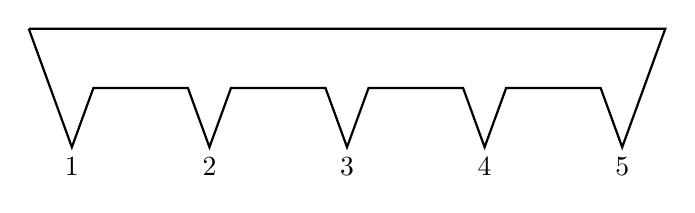
\begin{tikzpicture}[scale=.8]
\coordinate (O) at (0,0);
\draw [thick] (O) -- (++110:1cm) coordinate (P);
\draw[thick] (O) --
  ++(-70:1cm) coordinate(A) node[below] {$1$} -- 
  ++(+70:1cm) -- ++(0:1.5cm) --
  ++(-70:1cm) coordinate(B) node[below] {$2$} -- 
  ++(+70:1cm) -- ++(0:1.5cm) --
  ++(-70:1cm) coordinate(C) node[below] {$3$}-- 
  ++(+70:1cm) -- ++(0:1.5cm) --
  ++(-70:1cm) coordinate(D) node[below] {$4$} -- 
  ++(+70:1cm) -- ++(0:1.5cm) --
  ++(-70:1cm) coordinate(E) node[below] {$5$} --
  ++(+70:2cm) -- (P);

\end{tikzpicture}
\end{center}
\caption{A museum whose walls do not form a convex polygon}\label{f.museum.nonconvex}
\end{figure}

\begin{figure}[t]
\begin{center}
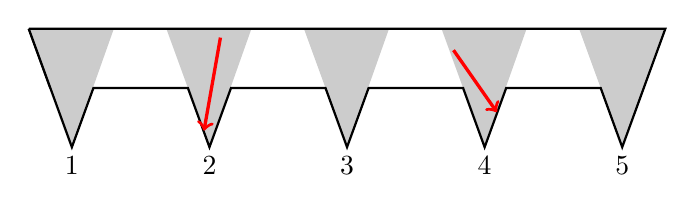
\begin{tikzpicture}[scale=.8]
\coordinate (O) at (0,0);
\draw [thick] (O) -- (++110:1cm) coordinate (P);
\path (O) --
  ++(-70:1cm) coordinate(A) node[below] {$1$} -- 
  ++(+70:1cm) coordinate(A1) -- ++(0:1.5cm) coordinate(A2) --
  ++(-70:1cm) coordinate(B) node[below] {$2$} -- 
  ++(+70:1cm) coordinate(B1) -- ++(0:1.5cm) coordinate(B2) --
  ++(-70:1cm) coordinate(C) node[below] {$3$}-- 
  ++(+70:1cm) coordinate(C1) -- ++(0:1.5cm) coordinate(C2) --
  ++(-70:1cm) coordinate(D) node[below] {$4$} -- 
  ++(+70:1cm) coordinate(D1) -- ++(0:1.5cm) coordinate(D2) --
  ++(-70:1cm) coordinate(E) node[below] {$5$} --
  ++(+70:2cm) coordinate(E1) -- (P);

\path[fill,black!20!white] (A) -- ++(110:2cm) -- ++(0:1.35cm)-- cycle;
\path[fill,black!20!white] (B) -- ++(110:2cm) -- ++(0:1.35cm)-- cycle;
\path[fill,black!20!white] (C) -- ++(110:2cm) -- ++(0:1.35cm)-- cycle;
\path[fill,black!20!white] (D) -- ++(110:2cm) -- ++(0:1.35cm)-- cycle;
\path[fill,black!20!white] (E) -- ++(110:2cm) -- ++(0:1.35cm)-- cycle;

\draw[thick] (P) -- (O) -- (A) -- (A1) -- (A2) --
   (B) -- (B1) -- (B2) -- (C) -- (C1) -- (C2) --
   (D) -- (D1) -- (D2) -- (E) -- (E1) -- (P);

\coordinate (G1) at (2.7,.8);
\coordinate (G2) at (6.4,.6);
\draw[->,red,very thick] (G1) -- +(-100:1.5cm);
\draw[->,red,very thick] (G2) -- +(-55:1.2cm);
\vertexcolor{G1}{red};
\vertexcolor{G2}{red};
\end{tikzpicture}
\end{center}
\caption{Visibility within each ``tooth''}\label{f.visibility-tooth}
\end{figure}

If at least one of the guards is placed near the top wall spanning the entire museum, she can observe all the horizontal walls (blue arrows in Fig.~\ref{f.museum.shaded}). Thus $5=15/3$ guards are sufficient to observe all the walls of the museum. Since the triangles do not overlap a guard in one triangle will not be able to observe all the walls of another triangle (green arrow) so $5$ guards are necessary.

\begin{figure}[ht]
\begin{center}
\begin{tikzpicture}[scale=.8]
\coordinate (O) at (0,0);
\draw [thick] (O) -- (++110:1cm) coordinate (P);
\path (O) --
  ++(-70:1cm) coordinate(A) node[below] {$1$} -- 
  ++(+70:1cm) coordinate(A1) -- ++(0:1.5cm) coordinate(A2) --
  ++(-70:1cm) coordinate(B) node[below] {$2$} -- 
  ++(+70:1cm) coordinate(B1) -- ++(0:1.5cm) coordinate(B2) --
  ++(-70:1cm) coordinate(C) node[below] {$3$}-- 
  ++(+70:1cm) coordinate(C1) -- ++(0:1.5cm) coordinate(C2) --
  ++(-70:1cm) coordinate(D) node[below] {$4$} -- 
  ++(+70:1cm) coordinate(D1) -- ++(0:1.5cm) coordinate(D2) --
  ++(-70:1cm) coordinate(E) node[below] {$5$} --
  ++(+70:2cm) coordinate(E1) -- (P);

\path[fill,black!20!white] (A) -- ++(110:2cm) -- ++(0:1.35cm)-- cycle;
\path[fill,black!20!white] (B) -- ++(110:2cm) -- ++(0:1.35cm)-- cycle;
\path[fill,black!20!white] (C) -- ++(110:2cm) -- ++(0:1.35cm)-- cycle;
\path[fill,black!20!white] (D) -- ++(110:2cm) -- ++(0:1.35cm)-- cycle;
\path[fill,black!20!white] (E) -- ++(110:2cm) -- ++(0:1.35cm)-- cycle;

\draw[thick] (P) -- (O) -- (A) -- (A1) -- (A2) --
   (B) -- (B1) -- (B2) -- (C) -- (C1) -- (C2) --
   (D) -- (D1) -- (D2) -- (E) -- (E1) -- (P);

\coordinate (G1) at (9,.8);
\coordinate (G2) at ($(O)+(.5,.5)$);
\draw[->,very thick,green!80!black,dashed] (G1) -- +(-165:4.6cm);
\draw[->,very thick,blue] (G2) -- ++(7.4,.35);
\draw[->,very thick,blue] (G2) -- ++(2.9,-.42);
\draw[thick] (6,0) circle(4pt);
\draw[thick] (4.95,-.28) circle(4pt);
\vertexcolor{G1}{green!80!black};
\vertexcolor{G2}{blue};
\end{tikzpicture}
\end{center}
\caption{Visibility of the walls of the museum}\label{f.museum.shaded}
\end{figure}

The example in Fig.~\ref{f.museum.nonconvex} can be generalized to $n/3$ teeth with $n$ walls, so we conclude that \emph{at least} $n/3$ guards are necessary. We wish to prove that $n/3$ guards are sufficient to guard any museum.

Section~\ref{s.museum-triangulating} proves that any triangulated polygon can be three-colored. This is used in Sect.~\ref{s.museum-guard} to prove the theorem that $n/3$ guards are sufficient. Section~\ref{s.museum-triangulated} completes the proof by showing that any polygon can be triangulated.

\section{Coloring Triangulated Polygons}\label{s.museum-triangulating}

\begin{definition}
A \emph{diagonal} a of polygon is an edge connecting two vertices that is not one of the (outside) edges of the polygon.
\end{definition}

\begin{definition} A polygon can be \emph{triangulated} if non-intersecting diagonals can be constructed such that the interior of the polygon is covered by triangles.
\end{definition}\index{Polygon!triangulated}
\vspace{-2ex}
\begin{theorem}
Any polygon can be triangulated.\label{thm.tri}
\end{theorem}
We defer the proof of Thm.~\ref{thm.tri}.
\begin{definition}
A vertex of a polygon is \emph{convex}\index{Polygon!convex and concave vertices} if its interior angle is less than $180^\circ$; a vertex is \emph{concave} if its interior angle is greater than $180^\circ$. 
\end{definition}
In Fig.~\ref{f.museum.arbitrary} vertex $1$ is convex and vertex $2$ is concave.

\begin{figure}[ht]
\begin{center}
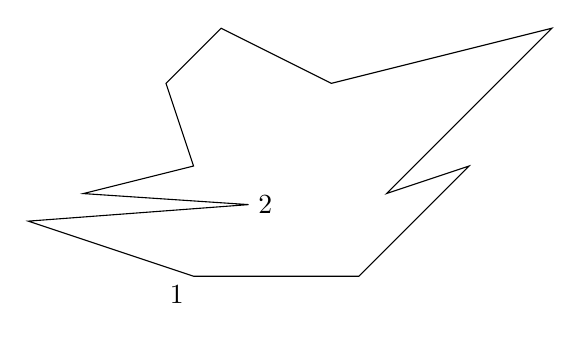
\begin{tikzpicture}[scale=.7]
\draw
  (0,0) coordinate (A) node[below left] {$1$} -- 
  ++(3,0) coordinate (B) --
  ++(2,2) coordinate (C) --
  ++(-1.5,-.5) coordinate (D) --
  ++(3,3) coordinate (E) -- 
  ++(-4,-1) coordinate (F) --
  ++(-2,1) coordinate (G) --
  ++(-1,-1) coordinate (H) --
  ++(.5,-1.5) coordinate (I) --
  ++(-2,-.5) coordinate (J) --
  ++(3,-.2) coordinate (K) node[right] {$2$} -- 
  ++(-4,-.3) coordinate (L) --
  cycle;
\vertex{A};
\vertex{K};
\end{tikzpicture}
\end{center}
\caption{A polygon with a convex vertex ($1$) and a concave vertex ($2$)}\label{f.museum.arbitrary}
\end{figure}

\begin{definition}
A polygon with vertices $V$ can be \emph{three-colored} if there is a map:
\[c: V \mapsto \{\mathit{red},\mathit{blue},\mathit{green}\}\,,\] such that no edge has two vertices that are assigned the same color.
\end{definition}

\begin{theorem}
A triangulated polygon can be three-colored.\label{thm.colored}
\end{theorem}\index{Coloring!polygon@of a polygon}

\begin{proof}
By induction on the number of vertices. A triangle can be three-colored. A triangulated polygon with $n>3$ vertices must have a diagonal. Choose an arbitrary diagonal $\overline{AB}$ (Fig.~\ref{f.museum.three-1}) and divide the polygon along this diagonal into two smaller polygons (Fig.~\ref{f.museum.three-2}). By induction each of these smaller polygons can be three-colored (Fig.~\ref{f.museum.three-3}).

Since the colors assigned are arbitrary, if different colors are assigned to $A,B$ in the two polygons, we can rename the colors in one of them so that the colors of $A,B$ are the same in both polygons. For example, in Fig.~\ref{f.museum.three-4} exchange \emph{red} and \emph{green} in the lower polygon.
Paste the two polygons together to recover the original polygon with $n$ vertices. It will be three-colored (Fig.~\ref{f.museum.three-5}).
\end{proof}

\begin{figure}[t]
\subfigures
\leftfigure[c]{
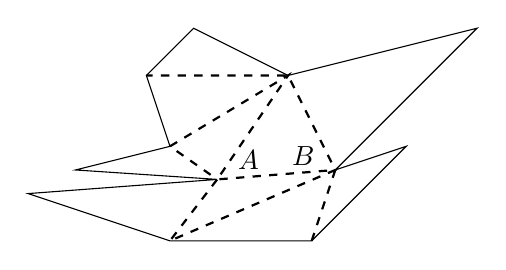
\begin{tikzpicture}[scale=.6]
\draw
  (0,0) coordinate (A) -- 
  ++(3,0) coordinate (B) --
  ++(2,2) coordinate (C) --
  ++(-1.5,-.5) coordinate (D) --
  ++(3,3) coordinate (E) -- 
  ++(-4,-1) coordinate (F) --
  ++(-2,1) coordinate (G) --
  ++(-1,-1) coordinate (H) --
  ++(.5,-1.5) coordinate (I) --
  ++(-2,-.5) coordinate (J) --
  ++(3,-.2) coordinate (K) -- 
  ++(-4,-.3) coordinate (L) --
  cycle;
\vertex{K};
\vertex{D};
\node[above right,xshift=4pt] at (K) {$A$};
\node[above left,xshift=-4pt,yshift=-2pt] at (D) {$B$};

\draw[thick,dashed]
  (B) -- (D) -- (K) -- (F) -- (I) -- (K) -- (A) -- (D) -- (F) -- (H);
\end{tikzpicture}
}
\hfill
\rightfigure[c]{
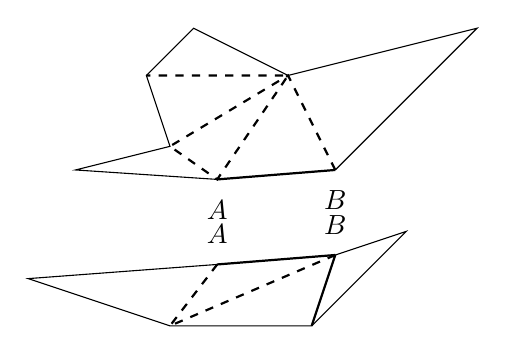
\begin{tikzpicture}[scale=.6]
\path
  (0,0) coordinate (A1) -- 
  ++(3,0) coordinate (B1) --
  ++(2,2) coordinate (C1) --
  ++(-1.5,-.5) coordinate (D1);
\draw
  (D1) --
  ++(3,3) coordinate (E1) -- 
  ++(-4,-1) coordinate (F1) --
  ++(-2,1) coordinate (G1) --
  ++(-1,-1) coordinate (H1) --
  ++(.5,-1.5) coordinate (I1) --
  ++(-2,-.5) coordinate (J1) --
  ++(3,-.2) coordinate (K1);
\path
  (K1) -- 
  ++(-4,-.3) coordinate (L1) --
  (A1);
\vertex{K1};
\vertex{D1};
\node[below,yshift=-4pt] at (K1) {$A$};
\node[below,yshift=-4pt] at (D1) {$B$};

\draw[thick,dashed]
  (D1) -- (F1) -- (I1) -- (K1) -- (F1) -- (H1);
\draw[thick] (D1) -- (K1);


\begin{scope}[yshift=-1.8cm]

\draw
  (0,0) coordinate (A2) -- 
  ++(3,0) coordinate (B2) --
  ++(2,2) coordinate (C2) --
  ++(-1.5,-.5) coordinate (D2);
\path
  (D2) --
  ++(3,3) coordinate (E2) --
  ++(-4,-1) coordinate (F2) --
  ++(-2,1) coordinate (G2) --
  ++(-1,-1) coordinate (H2) --
  ++(.5,-1.5) coordinate (I2) --
  ++(-2,-.5) coordinate (J2) --
  ++(3,-.2) coordinate (K2);
\draw
  (K2) --
  ++(-4,-.3) coordinate (L2) --
  (A2);
\vertex{K2};
\vertex{D2}; 
\node[above,yshift=4pt] at (K2) {$A$};
\node[above,yshift=4pt] at (D2) {$B$};

\draw[thick,dashed]
  (K2) -- (A2) -- (D2) -- (B2) -- (D2);
\draw[thick] (D2) -- (K2);

\end{scope}
\end{tikzpicture}
}
\leftcaption{An arbitrary diagonal in a polygon}\label{f.museum.three-1}
\rightcaption{Divide the polygon}\label{f.museum.three-2}
\end{figure}


\begin{figure}[t]
\subfigures
\leftfigure[c]{
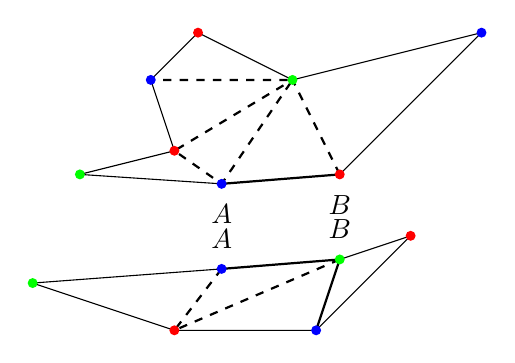
\begin{tikzpicture}[scale=.6]
\path
  (0,0) coordinate (A1) -- 
  ++(3,0) coordinate (B1) --
  ++(2,2) coordinate (C1) --
  ++(-1.5,-.5) coordinate (D1);
\draw
  (D1) --
  ++(3,3) coordinate (E1) -- 
  ++(-4,-1) coordinate (F1) --
  ++(-2,1) coordinate (G1) --
  ++(-1,-1) coordinate (H1) --
  ++(.5,-1.5) coordinate (I1) --
  ++(-2,-.5) coordinate (J1) --
  ++(3,-.2) coordinate (K1);
\path
  (K1) -- 
  ++(-4,-.3) coordinate (L1) --
  (A1);
  
\draw[thick,dashed]
  (D1) -- (F1) -- (I1) -- (K1) -- (F1) -- (H1);
\draw[thick] (D1) -- (K1);

\node[below,yshift=-4pt] at (K1) {$A$};
\node[below,yshift=-4pt] at (D1) {$B$};

\foreach \point/\color in {D1/red,E1/blue,F1/green,G1/red,H1/blue,I1/red,J1/green,K1/blue}
  \fill[color=\color] (\point) circle(3pt);

\begin{scope}[yshift=-1.8cm]

\draw
  (0,0) coordinate (A2) -- 
  ++(3,0) coordinate (B2) --
  ++(2,2) coordinate (C2) --
  ++(-1.5,-.5) coordinate (D2);
\path
  (D2) --
  ++(3,3) coordinate (E2) --
  ++(-4,-1) coordinate (F2) --
  ++(-2,1) coordinate (G2) --
  ++(-1,-1) coordinate (H2) --
  ++(.5,-1.5) coordinate (I2) --
  ++(-2,-.5) coordinate (J2) --
  ++(3,-.2) coordinate (K2);
\draw
  (K2) --
  ++(-4,-.3) coordinate (L2) --
  (A2);
  
\draw[thick,dashed]
  (K2) -- (A2) -- (D2) -- (B2) -- (D2);
\draw[thick] (D2) -- (K2);
\node[above,yshift=4pt] at (K2) {$A$};
\node[above,yshift=4pt] at (D2) {$B$};

\foreach \point/\color in {A2/red,B2/blue,C2/red,D2/green,K2/blue,L2/green}
  \fill[color=\color] (\point) circle(3pt);

\end{scope}
\end{tikzpicture}
}
\hfill
\rightfigure[c]{
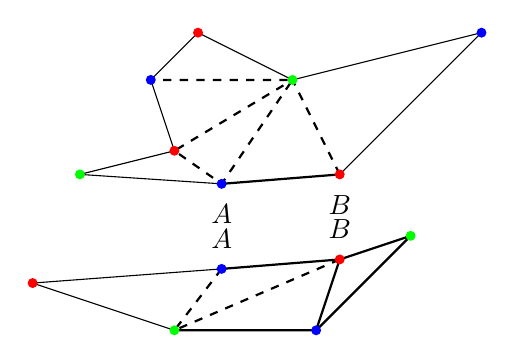
\begin{tikzpicture}[scale=.6]
\path
  (0,0) coordinate (A1) -- 
  ++(3,0) coordinate (B1) --
  ++(2,2) coordinate (C1) --
  ++(-1.5,-.5) coordinate (D1);
\draw
  (D1) --
  ++(3,3) coordinate (E1) -- 
  ++(-4,-1) coordinate (F1) --
  ++(-2,1) coordinate (G1) --
  ++(-1,-1) coordinate (H1) --
  ++(.5,-1.5) coordinate (I1) --
  ++(-2,-.5) coordinate (J1) --
  ++(3,-.2) coordinate (K1);
\path
  (K1) -- 
  ++(-4,-.3) coordinate (L1) --
  (A1);
  
\node[below,yshift=-4pt] at (K1) {$A$};
\node[below,yshift=-4pt] at (D1) {$B$};

\draw[thick,dashed]
  (D1) -- (F1) -- (I1) -- (K1) -- (F1) -- (H1);
\draw[thick] (D1) -- (K1);

\foreach \point/\color in {D1/red,E1/blue,F1/green,G1/red,H1/blue,I1/red,J1/green,K1/blue}
  \fill[color=\color] (\point) circle(3pt);

\begin{scope}[yshift=-1.8cm]

\draw[thick]
  (0,0) coordinate (A2) -- 
  ++(3,0) coordinate (B2) --
  ++(2,2) coordinate (C2) --
  ++(-1.5,-.5) coordinate (D2);
\path
  (D2) --
  ++(3,3) coordinate (E2) --
  ++(-4,-1) coordinate (F2) --
  ++(-2,1) coordinate (G2) --
  ++(-1,-1) coordinate (H2) --
  ++(.5,-1.5) coordinate (I2) --
  ++(-2,-.5) coordinate (J2) --
  ++(3,-.2) coordinate (K2);
\draw
  (K2) --
  ++(-4,-.3) coordinate (L2) --
  (A2);
  
\draw[thick,dashed]
  (K2) -- (A2) -- (D2) -- (B2) -- (D2);
\draw[thick] (D2) -- (K2);
\node[above,yshift=4pt] at (K2) {$A$};
\node[above,yshift=4pt] at (D2) {$B$};

\foreach \point/\color in {A2/green,B2/blue,C2/green,D2/red,K2/blue,L2/red}
  \fill[color=\color] (\point) circle(3pt);

\end{scope}
\end{tikzpicture}
}
\leftcaption{Three-color the two smaller polygons}\label{f.museum.three-3}
\rightcaption{Exchange the colors of one polygon to match the other}\label{f.museum.three-4}
\end{figure}

\begin{figure}[t]
\begin{center}
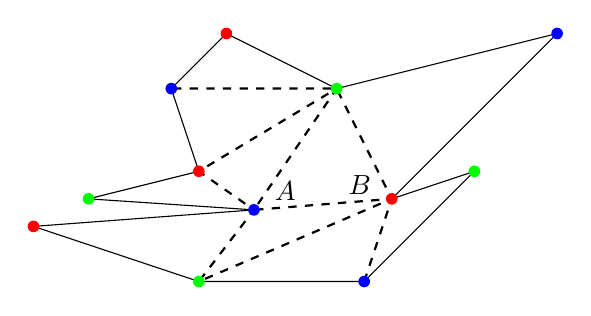
\begin{tikzpicture}[scale=.7]
\draw
  (0,0) coordinate (A) -- 
  ++(3,0) coordinate (B) --
  ++(2,2) coordinate (C) --
  ++(-1.5,-.5) coordinate (D) --
  ++(3,3) coordinate (E) -- 
  ++(-4,-1) coordinate (F) --
  ++(-2,1) coordinate (G) --
  ++(-1,-1) coordinate (H) --
  ++(.5,-1.5) coordinate (I) --
  ++(-2,-.5) coordinate (J) --
  ++(3,-.2) coordinate (K) -- 
  ++(-4,-.3) coordinate (L) --
  cycle;
  
\node[above right,xshift=4pt] at (K) {$A$};
\node[above left,xshift=-4pt,yshift=-2pt] at (D) {$B$};

\draw[thick,dashed]
  (B) -- (D) -- (K) -- (F) -- (I) -- (K) -- (A) -- (D) -- (F) -- (H);

\foreach \point/\color in {D/red,E/blue,F/green,G/red,H/blue,I/red,J/green,K/blue,A/green,B/blue,C/green,L/red}
  \fill[color=\color] (\point) circle(3pt);

\end{tikzpicture}
\end{center}
\caption{Paste the two smaller polygons back together}\label{f.museum.three-5}
\end{figure}

\newpage

\section{From Coloring of Polygons to Guarding a Museum}\label{s.museum-guard}

\begin{theorem}\label{thm.guarded} A museum with $n$ walls can be guarded by $n/3$ guards.
\end{theorem}\index{Museum!triangulated@and triangulated polygons}
\begin{proof}
By Thm.~\ref{thm.tri} the polygon can be triangulated and by Thm.~\ref{thm.colored} the polygon can be three-colored. All three vertices of each triangle in the triangulation must be colored by \emph{different} colors in order to satisfy the condition of being three-colored. Since the polygon is three-colored, at least one color, say red, can appear at most $n/3$ times, and every triangle must have a vertex colored red. Station a guard at each red vertex; she can observe all the walls of the each triangle the vertex belongs to. Since the triangles of the triangulation include all the edges of the polygon, $n/3$ guards are sufficient to observe all the walls of the museum.
\end{proof}
If $n$ is not divisible by $3$ the number of guards needed is $\lfloor n/3\rfloor$, the largest integer less than or equal to $n/3$. For example, $4$ guards are sufficient for museums with $12, 13, 14$ walls since $\lfloor 12/3\rfloor =\lfloor 13/3\rfloor=\lfloor 14/3\rfloor=4$. For simplicity we ignore this complication.
 
\section{Any Polygon Can Be Triangulated}\label{s.museum-triangulated}

\begin{theorem}\label{thm.interior-angles-of-a-polygon}
The sum of the interior angles of a polygon with $n$ vertices is:
\[180^\circ(n-2)\,.\]
\end{theorem}\index{Polygon!triangulated}
\begin{proof}
Consider a convex polygon and denote its \emph{exterior angles} by $\theta_i$ (Fig.~\ref{f.museum.exterior}).
As you move from one dashed line in sequence to the next dashed line, you complete a rotation around a circle so:
\[
\sum_{i=1}^n \theta_i = 360^\circ\,.
\]
\begin{figure}[t]
\begin{center}
\begin{tikzpicture}[scale=.5]
\coordinate (O) at (0,0);
\foreach \x/\name/\n/\po in {0/a/A/right,.6/b/B/above,1.6/c/C/left,2.4/d/D/below left,3.9/e/E/below right} {
  \coordinate (\name) at ($(O)+(\x*72+18:3cm)$);
}
\draw[thick] (a) -- (b) -- (c) -- (d) --(e) -- cycle;

\draw[thick,dashed] (a) 
  node[above,xshift=-2pt,yshift=8pt] {$\theta_1$} -- 
  ($(a)!2!(b)$);
\draw[thick,dashed] (b)
  node[above left,xshift=-8pt,yshift=0pt] {$\theta_2$} -- 
  ($(b)!1.7!(c)$);
\draw[thick,dashed] (c) 
  node[below left,xshift=-4pt,yshift=-2pt] {$\theta_3$} -- 
  ($(c)!1.7!(d)$);
\draw[thick,dashed] (d)
  node[below right,xshift=0pt,yshift=-4pt] {$\theta_4$} -- 
  ($(d)!1.5!(e)$);
\draw[thick,dashed] (e)
  node[right,xshift=4pt,yshift=4pt] {$\theta_5$} -- 
  ($(e)!1.7!(a)$);

\end{tikzpicture}
\end{center}
\caption{The exterior angles of a convex polygon}\label{f.museum.exterior}
\end{figure}
For each exterior angle $\theta_i$ denote its corresponding interior angle by $\phi_i$. Then:
\begin{eqnarray*}
\displaystyle\sum_{i=1}^n \theta_i &=&\displaystyle\sum_{i=1}^n (180^\circ-\phi_i)= 360^\circ\\
\displaystyle\sum_{i=1}^n \phi_i &=& n\cdot 180^\circ-360^\circ =180^\circ(n-2)\,.
\end{eqnarray*}
If there is a concave vertex ($B$ in Fig.~\ref{f.museum.concave}), there is a triangle formed by the two edges incident with the concave vertex and the line $\overline{AC}$ connecting the other two vertices. By summing the angles of the triangle we get:
\begin{eqnarray*}
(180^\circ - \alpha) + (360^\circ - \beta) + (180^\circ - \gamma) &=& 180^\circ\\
\alpha + \beta + \gamma &=& 3\cdot 180^\circ\,.
\end{eqnarray*}

The sum of the interior angles increases by $\alpha+\beta+\gamma$ while the number of vertices increases by three preserving the equation in the theorem:
\begin{eqnarray*}
\displaystyle\sum_{i=1}^n \phi_i + (\alpha + \beta + \gamma) &=& 180^\circ(n-2)+3\cdot 180^\circ\\
&=& 180^\circ((n+3)-2)\,.
\end{eqnarray*}
\end{proof}

\begin{figure}[t]
\begin{center}
\begin{tikzpicture}[scale=.8]
\draw[thick] (0,0) -- 
  (3,0) coordinate (A) node[above left,yshift=8pt] {$\alpha$} --
  ++(60:2) coordinate (B) node[above,yshift=8pt] {$\beta$} --
  ++(-60:2) coordinate (C) 
    node[above right,yshift=8pt] {$\gamma$}  --
  ++(3,0);

\draw ($(A)+(-.4,0)$) arc(180:60:.4);
\draw ($(B)+(-60:.3)$) arc(-60:240:.3);
\draw ($(C)+(.4,0)$) arc(0:120:.4);
\node[below] at (A) {$A$};
\node[below,yshift=-5pt] at (B) {$B$};
\node[below] at (C) {$C$};
\draw[thick,dashed] (A) -- (C);
\end{tikzpicture}
\end{center}
\caption{A concave vertex}\label{f.museum.concave}
\end{figure}


\begin{theorem}\label{thm.convex}
There must be at least three convex vertices in a polygon.
\end{theorem}

\begin{proof} Let $k$ be the number of concave vertices where the interior angle of each is $180^\circ+\epsilon_i$, $\epsilon_i>0$. The sum of the interior angles of the \emph{concave} vertices is certainly less than or equal to the sum of the interior angles of \emph{all} the vertices:
%
\begin{eqnarray*}
k\cdot 180^\circ +\displaystyle\sum_{i=1}^{k}\epsilon_i &\leq& 180^\circ(n-2)\\
(k+2)\cdot 180^\circ +\displaystyle\sum_{i=1}^{k}\epsilon_i &\leq& n\cdot 180^\circ\\
(k+2)\cdot 180^\circ &<& n\cdot 180^\circ\\
k&<&n-2\,.
\end{eqnarray*}
It follows that there must at least three vertices that are convex, not concave.
\end{proof}

\begin{proof}[Theorem~\ref{thm.tri}]
By induction on the number of vertices. For $n=3$ there is nothing to prove. If $n>3$, by Thm.~\ref{thm.convex} there must be a convex vertex $C$. Label its adjacent vertices by $B,D$. If $\overline{BD}$ is contained within the polygon (Fig.~\ref{f.contained}), it is a diagonal and the polygon can be split into $\triangle BCD$ and another polygon $\overline{ABDE}$ with $\overline{BD}$ as an edge and which is smaller than the original polygon (Fig.~\ref{f.contained}). By the inductive hypothesis, the polygon can be triangulated and then pasted back to $\triangle BCD$, triangulating the original polygon.

\begin{figure}[t]
\subfigures
\leftfigure[c] {
\begin{tikzpicture}[scale=1.4]
\clip (-.5,-.4) rectangle (3.8,2.2);
\draw
  (0,0) coordinate (A) -- 
  ++(1.5,0) coordinate (B) --
  ++(2,2) coordinate (C) --
  ++(-1.8,-.5) coordinate (D) --
  ++(-1,.5) coordinate (E) --
  (A);
\draw[thick,dashed] (B) -- (D);
\foreach \point/\pos in {A/below,B/below,C/right,D/above,E/left}
  \node[\pos] at (\point) {$\point$};
\vertex{B};
\vertex{D};
\end{tikzpicture}
}
\hfill
\rightfigure[c] {
\begin{tikzpicture}[scale=1.4]
\clip (-.2,-.4) rectangle (3.8,2.2);
\draw
  (0,0) coordinate (A) -- 
  ++(1.5,0) coordinate (B) --
  ++(2,2) coordinate (C) --
  ++(-1.8,-.5) coordinate (D) --
  ++(-1,.5) coordinate (E) --
  ++(1.3,-1) coordinate (F) --
  (A);
\draw[thick,dashed] (B) -- (D);
\draw[very thick,dotted] (C) -- (F);
\node [draw,circle through=(F)] at (C) {};
\node[below] at (A) {$A$};
\node[below] at (B) {$B$};
\node[right] at (C) {$C$};
\node[above,yshift=2pt,xshift=-3pt] at (D) {$D$};
\node[left]  at (E) {$E$};
\node[below,yshift=-1pt,xshift=-2pt] at (F) {$F$};
\vertex{C};
\vertex{F};
\end{tikzpicture}
}
\leftcaption{Triangulation where a diagonal is contained within the polygon}\label{f.contained}
\rightcaption{Triangulation where a diagonal is not contained within the polygon}\label{f.museum.concave-vertices}
\end{figure}
If $\overline{BD}$ is not contained in the polygon, there must be concave vertex $F$ that is \emph{closest} to $C$ (Fig.~\ref{f.museum.concave-vertices}). $\overline{CF}$ is a diagonal and splits the polygon into two smaller polygons $\overline{CFED}$ and $\overline{CFAB}$. By the inductive hypothesis these can be triangulated and pasted together.
\end{proof}

\subsection*{What Is the Surprise?}
The museum theorem is suprising because what seems to be a theorem in geometry is proved rather elegantly by an appeal to coloring a graph.

\subsection*{Sources}

This chapter is based on \cite[Chap.~39]{thebook}.
